% !TEX program = pdflatex
% !TEX enableSynctex = true


        %%%%%%%%%%%%%%%%%%%%%%%%%%%%%%%%%%%%%%%%%%%%%%%%%%%%%%%%%%%%%%%%%%%%%%%%%%%%%%%%%%%%
        \documentclass[12pt]{article}
        \usepackage[margin=1in]{geometry} 
        \usepackage[hidelinks]{hyperref}
       \usepackage{amsmath,amsthm,amssymb,amsfonts, enumitem, fancyhdr, color, comment, graphicx, environ,mathtools, bbm, tikz, setspace, cleveref,listings, dcolumn, xcolor}
       
       \usepackage[T1]{fontenc}
       
       \usepackage{array, multirow, caption, booktabs}
       \usepackage{ mathrsfs }
       \hypersetup{
           colorlinks,
           linkcolor={red!50!black},
           citecolor={blue!50!black},
           urlcolor={blue!80!black}
       }
       \usetikzlibrary{matrix,positioning}
       \tikzset{bullet/.style={circle,draw=black,inner sep=8pt}}
       \DeclareMathOperator*{\argmax}{arg\,max}
       \DeclareMathOperator*{\argmin}{arg\,min}
       \DeclareMathOperator*{\Var}{\text{Var}}
       \DeclareMathOperator*{\Cov}{\text{Cov}}
       
       \DeclarePairedDelimiter\norm{\lVert}{\rVert}%
       \newtheorem{theorem}{Theorem}
       \newtheorem{lemma}[theorem]{Lemma}
       \DeclareMathOperator{\eps}{\varepsilon}
       \doublespacing
       \DeclarePairedDelimiter\abs{\lvert}{\rvert}%
       \pagestyle{fancy}
       \setlength{\headheight}{65pt}
       \newenvironment{problem}[2][Problem]{\begin{trivlist}
       \item[\hskip \labelsep {\bfseries #1}\hskip \labelsep {\bfseries #2.}]}{\end{trivlist}}
       \newenvironment{sol}
           {\emph{Solution:}
           }
           {
           \qed
           }
       
       \lstdefinelanguage{Julia}%
         {morekeywords={abstract,break,case,catch,const,continue,do,else,elseif,%
             end,export,false,for,function,immutable,import,importall,if,in,%
             macro,module,otherwise,quote,return,switch,true,try,type,typealias,%
             using,while},%
          sensitive=true,%
          alsoother={$},%
          morecomment=[l]\#,%
          morecomment=[n]{\#=}{=\#},%
          morestring=[s]{"}{"},%
          morestring=[m]{'}{'},%
       }[keywords,comments,strings]%
       
       \lstset{%
           language         = Julia,
           basicstyle       = \ttfamily,
           keywordstyle     = \bfseries\color{blue},
           stringstyle      = \color{magenta},
           commentstyle     = \color{ForestGreen},
           showstringspaces = false,
       }
       
       
       %%%%%%%%%%%%%%%%%%%%%%%%%%%%%%%%%%%%%%%%%%%%%%%%%%%%%%%%%%%%%%%%%%%%%%%%%%%%%%%%%
       
       
       \usepackage{xcolor}
        
       \definecolor{codegreen}{rgb}{0,0.6,0}
       \definecolor{codegray}{rgb}{0.5,0.5,0.5}
       \definecolor{codepurple}{rgb}{0.58,0,0.82}
       \definecolor{backcolour}{rgb}{0.95,0.95,0.92}
        
       \lstdefinestyle{mystyle}{
           backgroundcolor=\color{backcolour},   
           commentstyle=\color{codegreen},
           keywordstyle=\color{magenta},
           numberstyle=\tiny\color{codegray},
           stringstyle=\color{codepurple},
           basicstyle=\ttfamily\footnotesize,
           breakatwhitespace=false,         
           breaklines=true,                 
           captionpos=b,                    
           keepspaces=true,                 
           numbers=left,                    
           numbersep=5pt,                  
           showspaces=false,                
           showstringspaces=false,
           showtabs=false,                  
           tabsize=2
       }
        
       \lstset{style=mystyle}    
       
       
       %%%%%%%%%%%%%%%%%%%%%%%%%%%%%%%%%%%%%%%%%%%%%
       
       \rhead{John Higgins\\Programming Bootcamp \\ 20 July, 2022} 
       
       %%%%%%%%%%%%%%%%%%%%%%%%%%%%%%%%%%%%%%%%%%%%%
       
       
       %%%%%%%%%%%%%%%%%%%%%%%%%%%%%%%%%%%%%%
       
       \begin{document}
       \lstset{language=Julia}
       %%%%%%%%%%%%%%%%%%%%%%
       Note: All code and plots can be found \href{https://github.com/johnfhiggins/Coding-Bootcamp/tree/main/PS4}{here!}
       \begin{problem}{1}
       
       \end{problem}
       \begin{sol}
        Code and putput for problem 1 is included below:
        \begin{lstlisting}
function matrix_fill(N::Int64, coins::Array{Int64})
    #initialize an empty array of size N+1 x the amount of coins + 1
    #note: because I need a row of ones at the beginning (so that successful ways of making change get counted), the indices of everything will be shifted up by 1. It's not pretty, but it works
    res = zeros(N+1, length(coins)+1)
    #create the aforementioned row of ones
    res[1, :] .= 1
    #sort the list of coins we have, because the way I have written it depends on the list of coins being ordered
    coins = sort(coins)
    #iteratively fill in the rows of the matrix 
    for val=1:N
        #iterate over possible coins to use
        for (i, coin) in enumerate(coins)
            if coin > val #if the coin is larger than the remaining balance
                res[val+1,i+1] = res[val+1, i] #we cannot make change using this coin, so we use the previous count for the first i-1 coins
            elseif coin == val #if the coin is exactly the same as the remaining balance
                res[val+1,i+1] = 1 + res[val+1, i] #use this coin to make exact change and thus we need to increment the current count by 1 
            else
                #can always make change with the lower denomination coins and ignore the new coin
                res[val+1,i+1] = res[val+1,i]
                #find the highest quantity of coin i that can be used 
                j_range = Int(floor(val/coin))
                #loop over possible multiples of the current coin, up to j_range
                for j=1:j_range
                    #add the number of ways to make change for the resulting balance with the first i-1 coins and add to the current entry 
                    res[val+1, i+1] += res[val + 1  - j*coin, i]
                end
            end
        end
    end
    #return the resulting matrix, as well as the total number of ways (it will be the entry in the bottom right corner of the matrix)
    res, res[N+1, length(coins)+1]
end 

#find the total amount of ways 
full_matrix, total_ways = matrix_fill(10, [2,3,5,6])
total_ways
>>5.0
        \end{lstlisting}
       \end{sol}
       \begin{problem}{2}
        
       \end{problem}
       \begin{sol}
        Code and output for problem 2 is included below:
        \begin{lstlisting}
#create bellman function for problem: takes rod length N and price vector P
function rod_bellman(N::Int64, P::Vector{Int64})
    #assign empty policy and value arrays
    value_mat = zeros(N)
    pol_func = zeros(N)
    #loop over state variables n 
    for n=1:N
        #start with the candidate choice being to just sell the remaining rod and the candidate max being the value of the remaining
        cand_pol = n
        cand_max = P[n]
        #loop over all rod lengths to cut off; since n is the default, it is not included here
        for i=1:n-1
            #value of choosing length i to cut off is the price of a rod of length i plus the continuation value at n-i
            val = P[i] + value_mat[n-i]
            #if we get a value higher than the candidate max (note: it is possible that there is a tie between two different policies - this doesn't really matter though since we are interested in maximizing the value)
            if val >= cand_max
                #update the max and argmax candidates
                cand_max = val
                cand_pol = i
            end
        end
        #find the value of having a rod of length n by choosing the above candidate 
        value_mat[n] = cand_max
        pol_func[n] = cand_pol 
    end
    #return the value and policy vectors
    value_mat, pol_func
end

function rod_solver(P::Vector{Int64})
    #start with price vector corresponding to rod of length N
    N = length(P)
    #initialize empty policy sequence
    pol_seq = []
    #fill in the value function and policy vectors 
    val, pol = rod_bellman(N, P)
    #use while loop to iteratively find the policy choices required to achieve the max value
    while N >= 1
        #find the policy function for a rod of length N
        cur_pol = Int(pol[N])
        #add the current policy to the policy sequence
        append!(pol_seq, cur_pol)
        #decrease N by the amount of the current policy
        N = N - cur_pol
    end
    #return the overall value as well as the sequence required to attain it
    val[length(P)],pol_seq
end

value_n, cuts = rod_solver( [1,5,8,9,10,17,17,20])
value_n
>>22.0
cuts
>>[6,2]

value_n, cuts = rod_solver( [1,5,45,9,10,17,17,20])
value_n
>>95.0
cuts
>>[3,3,2]
        \end{lstlisting}
       \end{sol}
       \begin{problem}{3}
        
       \end{problem}
       \begin{sol}
        Code and output for problem 3 is included below:
        \begin{lstlisting}
#note: I assume item array is ordered by ascending weight
function knap_bellman(values::Vector{Int64}, weights::Vector{Int64}, C::Int64)
    N = length(values)
    #create empty value array
    v_mat = zeros(N+1, C+1)
    #create empty weight array associated with the values in the value array
    w_mat = zeros(N+1,C+1)
    #create policy array which attains the values in the value array
    p_mat = fill([], N+1, C+1)
    for c=1:C+1
        for (i,item) in enumerate(values)
            #for convenience, define the weight and value of item i
            w_i = weights[i]
            v_i = values[i]
            if w_i > c #if i is not feasible, ignore it and set arrays to previous choice 
                v_mat[i+1,c] = v_mat[i, c]
                w_mat[i+1,c] = w_mat[i,c]
                w_mat[i+1, c] = w_mat[i, c]
            elseif w_i ==  c #if item i is exactly the weight limit
                if values[i] >= v_mat[i,c] #if i is better than the previous optimal choice
                    if weights[i] <= w_mat[i,c] #if i weighs less than the previous optimal choice, set values, weights, and policy so that i is chosen at weight c
                        p_mat = [i]
                        v_mat[i+1, c] = v_i
                        w_mat[i+1, c] = w_i
                    end
                end
            else
                #start with i being the candidate optimal choice
                cand_max = v_i
                cand_weight = w_i
                cand_pol = [i]
                for j=1:i-1 #loop over possible choices of smaller subsets
                    v_ij = v_i + v_mat[j+1, c-w_i] #the value of choosing i and the optimal choice of items (1,...,j) with weight at most c - w_i
                    w_ij = w_i+ w_mat[j+1, c-w_i]#weight of the above
                    #println(v_ij, " ", w_ij, " ", values[i], " ", v_mat[j+1, c-w_i+1], w_ij, c)
                    if w_ij <= c
                        if v_ij >= cand_max #if the value of using i with the optimal bundle of items (1,...,j) of weight less than c-w_i is greater than the candidate maximum, set the candidates equal to this new combination
                            cand_max = v_ij
                            cand_weight = w_ij
                            cand_pol = p_mat[j+1, c-w_i]
                        end
                    end
                end
                #set value and weight for optimal bundle of weight less than c which potentially includes up to item i
                v_mat[i+1, c] = cand_max
                w_mat[i+1, c] = cand_weight
                
                if cand_pol ==[i] #if we are sticking with policy i
                    p_mat[i+1, c] = cand_pol #set the policy to i
                else #if we are combining i with an existing policy vector
                    new_pol = copy(cand_pol)
                    append!(new_pol, i) #append to previous policy vector
                    p_mat[i+1, c] = new_pol #create entry for new policy vector
                end
            end
        end
    end
    #return value and optimal policy vector
    v_mat[N+1, C+1], p_mat[N+1, C+1]
end

#determine value and optimal policies
knap_bellman([4,3,8], [1,1,2], 3)
>> 12, [1,3]
knap_bellman([60,100,120], [10,20,30], 50)
>> 220, [2,3]
        \end{lstlisting}
To see how this is a generalization of the problem in part 2, we note that if we set C = 8 and the weight of a rod of length x to be x, then it is exactly the same problem. 
       \end{sol}
       \begin{problem}{4}
        
       \end{problem}
       \begin{sol}
        Suppose there is an infinitely-lived firm with discount factor $\beta$ which faces linear inverse demand $P(q) = a - b q$ in each period, where $q$ is the quantity supplied by the firm. The firm starts with marginal cost $c_0$ in period $t=0$. Each period, the firm can choose to invest in cost-reducing research. Specifically, if their marginal cost is $c_t$ in period $t$, investing $x_t$ dollars in research in period $t$ lowers their marginal cost in period $t+1$ to $c_{t+1} = f(c_t, x_t)$ for some function $f$ which is increasing in $c_t$ and decreasing in $x_t$. We specialize by using $f(c_t, x_t) = \alpha^{x_t} c_t $, where $\alpha \in (0,1)$. The firm's profit in period $t$ is given by
        \[\pi(q_t, x_t) = (P(q_t) - f(c_{t-1}, x_{t-1}))q_t - x_t\]
        However, we can consolidate this. If the firm wishes to transition from $c_t$ to $c_{t+1}$, they must pay an adjustment cost of $\Phi(c_{t}, c_{t+1}) = f^{-1}(c_{t}, c_{t+1})= \log_{\alpha}\left(\frac{c_{t+1}}{c_t} \right)$ when $c_{t+1} \geq c_t$ and $\Phi(c_t, c_{t+1}) = 0$ otherwise. Hence, the firm's period-$t$ profit given current cost $c_t$ and next period cost $c_{t+1}$ becomes
        \[\pi(q_t, c_t, c_{t+1}) = (P(q_t) - c_t)q_t - \Phi(c_t, c_{t+1})\]
        The firm's problem is thus to choose $\{q_t, c_{t+1}\}_{t=0}^{\infty}$ to solve
        \[\max_{\{q_t, c_{t+1}\}_{t=0}^{\infty}} \sum_{t=0}^{\infty} \beta^t \left[(P(q_t) - c_t)q_t - \Phi(c_t, c_{t+1})\right]\]
        subject to the constraints that $q_t, c_{t+1} \geq 0$ $\forall t$ and $c_{0} > 0$.
        Alternatively, we note that we can express the firm's problem in a recursive manner. The value function of the firm with current cost $c$ is given by 
        \[V(c) = \max_{q, c'} \left[\pi(q, c, c') + \beta V(c')\right]\]
        We focus first on the first order condition for $q$. Using that $P(q) = a - bq$, we find that the optimal quantity must solve 
        \[0 = a - 2bq - c  \iff q = \frac{a -c}{2b}\]
        This is independent of the choice of $c'$. Thus, a firm with cost $c$ will optimally set $q(c) = \frac{a-c}{2b}$. We can rewrite the firm's Bellman equation as follows:
        \[V(c) = \max_{c'} \left[\pi(q(c), c, c') + \beta V(c')\right]\]
        We can see now that this is a fixed point of the contraction mapping $T: f \rightarrow Tf$ where
        \[(T f)(c) = \max_{c'} \left[ \pi(q(c), c, c') + \beta f(c') \right]\]
        Thus, we can find the value function through value function iteration. We will do this in Julia. Julia code is included below, as well as graphs of value and policy functions for a selection of parameter values.
        \begin{center}
            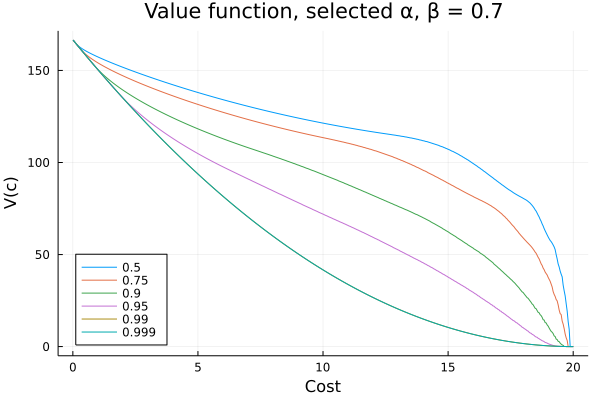
\includegraphics[scale=0.6]{vfplotbeta=7}
            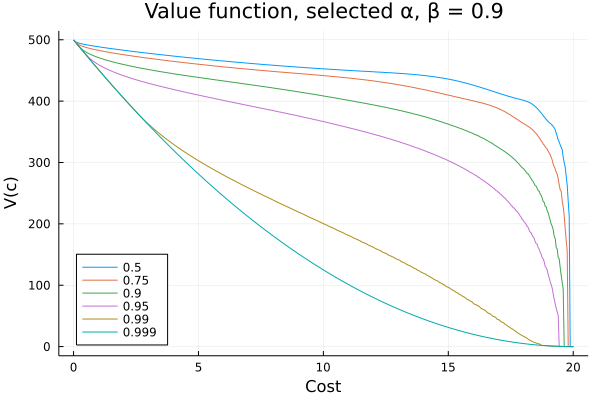
\includegraphics[scale=0.6]{vfplotbeta=9}
            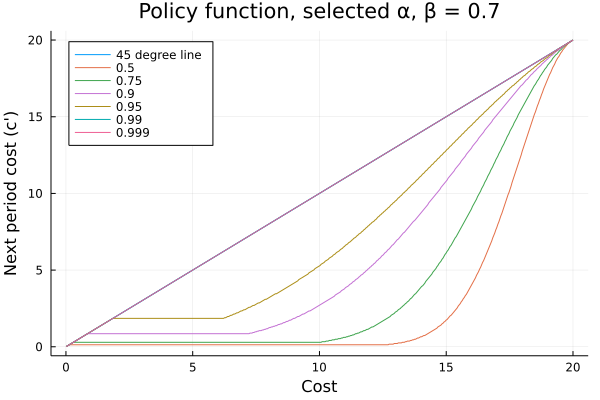
\includegraphics[scale=0.6]{pfplotbeta=7}
            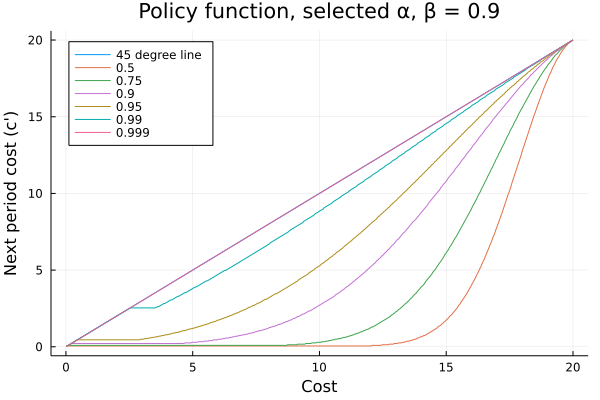
\includegraphics[scale=0.6]{pfplotbeta=9}
        \end{center}
        Notice that, as we would expect, a higher $\alpha$ leads firms to choose a lower cost in the next period (since a lower $\alpha$ makes cost-reduction less expensive). Furthermore, a higher discount factor $\beta$ leads firms to invest more in cost-reduction. We also include a plot showing the evolution of cost over time according to the policy functions we found above. Note that when the discount factor is higher, firms reduce cost quicker and further. When the discount factor is lower, firms are slower to reduce cost and end up reducing it less. We can deduce that the steady state cost is lower for firms which are more forward-looking.
        \begin{center}
            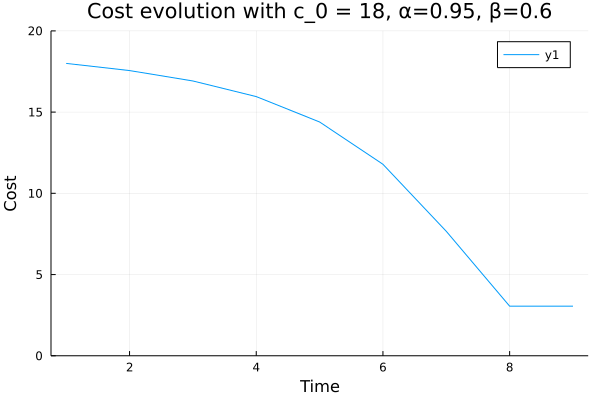
\includegraphics[scale=0.6]{costevol6}
            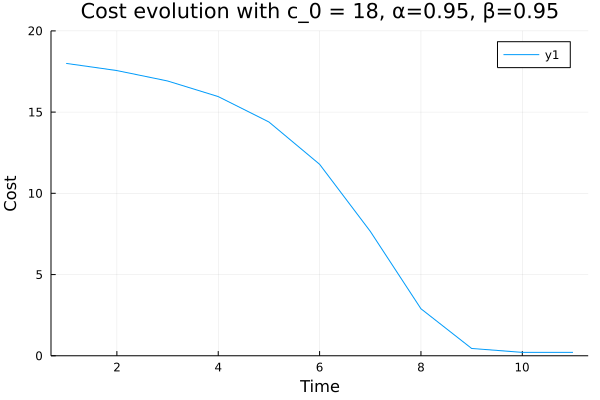
\includegraphics[scale=0.6]{costevol95}
        \end{center}
        \begin{lstlisting}
    using Parameters, Plots

@with_kw struct Primitives
    \beta::Float64 = 0.6 #discount rate
    a::Float64 = 20.0 #demand intercept
    b::Float64 = 2.0 ##demand slope

    alph::Float64 = 0.95 #research parameter, factor by which marginal cost is reduced

    c0::Float64 = 20.0 #max cost    
    c_grid::Vector{Float64} = collect(range(0.01, length=500, stop=c0)) #cost grid
    nc::Int64 = length(c_grid) #number of grid points
    #grid_gen(c_0, alph, nc)
end
mutable struct Results
    val_func::Array{Float64} #value function
    pol_func::Array{Float64} #policy function
end

function adj_cost(ct::Float64, ct1::Float64, alph::Float64)
    rat = ct1/ct #find ratio of future c to current c
    if rat >= 1 #if future cost greater than current
        val = 0 #no adjustment cost (no investment needed to produce at previous cost)
    else
        val = log(alph, rat) #find the amount which needs to be invested to achieve future cost
    end
    val #return adjustment cost
end

function obj_func(ct::Float64, ct1::Float64, a::Float64, b::Float64, alph::Float64)
    q = ((a-ct)/(2b)) #optimal quantity in each period
    rev = q*(a - b*q - ct) #profit at optimal quantity
    cost = adj_cost(ct, ct1, alph) #cost of new investment to get to next period cost ct1
    val = rev - cost #profit net investment cost
    if val < 0 ## impose condition that investment must be lower than current revenue by giving very low value when it is violated
        val = -10000
    end
    val
end
    #@unpack 

function Bellman(prim::Primitives, res::Results, alph::Float64)
    @unpack \beta, a, b,  c0, c_grid, nc = prim
    v_new = zeros(nc) #new policy function array
    for ci=1:nc #loop over cost index 
        c = c_grid[ci] #find corresponding cost
        cand_max = -50.0 #start with really bad value for max
        for i=1:nc #loop over index of next period's cost
            ct1 = c_grid[i] #find corresponding next period cost
            val = obj_func(c, ct1, a, b, alph) + \beta*res.val_func[i] #find value of choosing ct1 
            if val >= cand_max #check if this is better than the previous one; if so, update max candidates and policy function
                cand_max = val
                res.pol_func[ci] = ct1
            end
        end
        v_new[ci] = cand_max #fill in value function
    end
    v_new #return new value function
end


function model_solver(alpha::Float64)
    prim = Primitives()
    @unpack nc, c_grid, c0 = prim
    val_func, pol_func = zeros(nc), zeros(nc) #init blank value and policy function arrays 
    res = Results(val_func, pol_func) 
    tol = 0.0001 #tolerance param for convergence
    N = 1000 #max iterations
    n=0 
    error = 100 #starting error
    while error > tol && n < N #loop until convergence or max iterations reached
        n +=1
        v_new = Bellman(prim, res, alpha) #find new value function
        error = maximum(abs.(v_new - res.val_func)) #max difference between old value function and new value function
        println("Iteration ", n, ", error = ", error)
        res.val_func = v_new #update value function
    end
    println("Convergence!")

    #vfplot = plot(c_grid, res.val_func, title="Value") #plot value function
    #pfplot = plot(c_grid, [c_grid, res.pol_func], labels=[ "45 degree line" "Policy function"],title="Policy", ylims=(0,Int(c0))) #plot policy function and 45 degree line
    #display(vfplot)
    #display(pfplot)
    res.val_func, res.pol_func
end



function multiple_plots()
    @unpack c_grid , \beta = Primitives()
    alpha_list = [0.5, 0.75, 0.9, 0.95, 0.99, 0.999]
    #vf_arr = fill([], 5)
    #pf_arr = fill([], 5)
    vf_plot = plot()
    pf_plot = plot(c_grid, c_grid, title="Value function, selected \alpha", xlabel="Cost", ylabel="Next period cost", labels="45 degree line", legend=:topleft)
    for (i,al) in enumerate(alpha_list)
        vfa, pfa = model_solver(al)
        plot!(vf_plot, c_grid, vfa, title="Value function, selected \alpha, \beta = $(\beta)", xlabel="Cost", ylabel="V(c)", labels=al, legend=:bottomleft)
        plot!(pf_plot, c_grid,  pfa, title="Policy function, selected \alpha, \beta = $(\beta)", xlabel="Cost", ylabel="Next period cost (c')", labels = al, legend=:topleft)
        #vf_arr[i] = vfa
        #vf_arr[]
    end
    display(vf_plot)
    display(pf_plot)
    cd(dirname(@__FILE__())) 
    savefig(vf_plot, "vfplot beta=$(\beta).png")
    savefig(pf_plot, "pfplot beta=$(\beta).png")
end

function cost_evol()
    #cost evolution
    alph = 0.95
    @unpack c_grid, \beta = Primitives()
    vf, pf = model_solver(alph)
    
    ci = 450
    cs = [c_grid[ci]]
    vs = [vf[ci]]
    error = 100
    while error > 0.01
        c = c_grid[ci]
        ct1 = pf[ci]
        error = c - ct1
        push!(cs, ct1)
        ci = findfirst(isequal(ct1), c_grid)
        push!(vs, vf[ci])
    end
    plot_evol = plot(cs, title="Cost evolution with c_0 = 18, \alpha=$(alph), \beta=$(\beta)", xlabel="Time", ylim=(0,20), ylabel="Cost")
    savefig(plot_evol, "costevol$(\beta).png")
    #plot(vs)
end
        \end{lstlisting}
       \end{sol}
       \end{document}
       